\section{Zielsetzung}
\label{sec:Zielsetzung}

Ziel dieses Versuches ist es das Relaxationsverhalten eines RC-Kreises zu untersuchen. 
Dies erfolgt durch Bestimmung der Zeitkonstante, Messung der frequenzabhängigen Amplitude der Kondensatorspannung und 
der frequenzabhängigen Phasenverschiebung zwischen Generator- und Kondensatorspannung.
Außerdem wird gezeigt, dass der RC-Kreis als Integrator arbeiten kann.


\section{Theorie}
\label{sec:Theorie}

\subsection{Allgemeines Relaxationsverfahren} % (fold)
\label{sub:Allgemein}
Relaxation in der Physik ist das nicht-oszillatiorische Zurückkehren in den Ausgangszustand eines Systems, nachdem es daraus entfernt wurde.
Als Beispiel für das Relaxationsphänomen kann die Schaltung in \autoref{fig:Kondensator} benutzt werden. 
\begin{figure}[H]
    \centering
    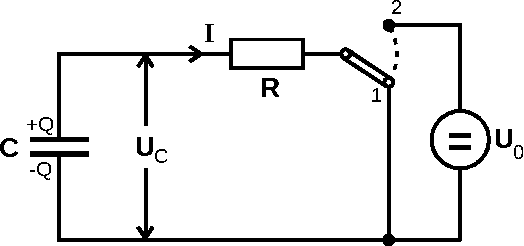
\includegraphics[width=0.5\textwidth]{build/Abb_1.pdf}
    \caption {Auf- und Endladung eines Kondensators über einen Widerstand.\cite{v353}}
    \label{fig:Freque_A&P_durch}
\end{figure}
\noindent Diese stellt die Auf- und Entladung des Kondensators über einen Widerstand dar.
Die Aufladevorgang beginnt beginnt, wenn der Schalter auf Position $2$ gestellt wird und der Entladevorgang beginnt, wenn der Schalter auf Position $1$ steht.
% subsection Allgemein (end)

\subsection{Entladevorgang eines Kondensators} % (fold)
\label{sub:Entladevorgang}
Der Entladevorgang beginnt, wenn sich auf dem Kondensator die Ladung $Q$ befindet.
Dann liegt zwischen den Platten die Spannung
\begin{equation}
    U_C = \frac{Q}{C}
\end{equation}
an und nach dem Ohmschen Gesetzt ergibt dies den Strom
\begin{equation}
    I = \frac{U_C}{R} .
\end{equation}
Der zeitliche Verlauf der Ladung lässt sich darstellen durch
\begin{equation}
    Q(t) = Q(0) e^{\frac{-1}{RC}}
\end{equation}
,wobei $RC$ eine Zeitkonstante ist, die im nächsten Kapitel näher erläutert wird.
% subsection Entladevorgang (end)


\subsection{Aufladevorgang eines Kondensators} % (fold)
\label{sub:Aufladevorgang}
Beim Aufladevorgang müssen die Ranbedingungen
\begin{align}
    Q(0)&=0 &\text{und}& Q(\infty)=CU_0
\end{align}
gelten. Der Aufladevorgang kann dann durch die Gleichung
\begin{equation}
    Q(t)= CU_0\Bigl(1-e^{\frac{-t}{RC}}\Bigr)
\end{equation}
dargestellt werden. Die Zeitkonstante ist auch hier wieder $RC$ ist.
Sie ist ein Geschwindigkeitsmaß mit dem das System seinem Endzustand (hier Q(\infty)) entgegen strebt.
Die Ladung auf dem Kondensator ändert sich um den Faktor
\begin{equation}
    \frac{Q(t)}{Q(0)} = \frac{-t}{RC}
\end{equation}
und für den Zeitraum $\Delta T = RC$ gilt
\begin{equation}
    \frac{Q(t)}{Q(0)} = \frac{1}{e} \approx 0,368 .
\end{equation}


% subsection Aufladevorgang (end)

\subsection{Relaxationsphänomen bei einer periodischen Auslenkung} % (fold)
\label{sub:Rela_peri}

% subsection Relaxationsphänomen bei einer periodischen Auslenkung (end)

\subsection{Der RC-Kreis als Integrator} % (fold)
\label{sub:Integrator4}

% subsection  (end)

